\section{Electrostatic Lens}

\subsection{Testing procedure}

\subsection{Simulations}

\subsection{Vacuum chambers for testing}

\subsection{HV connections}

\subsection{Electrode conditioning at HV}

\subsection{Re-entrant flanges for detection}

\begin{figure}[b]
    \centering
    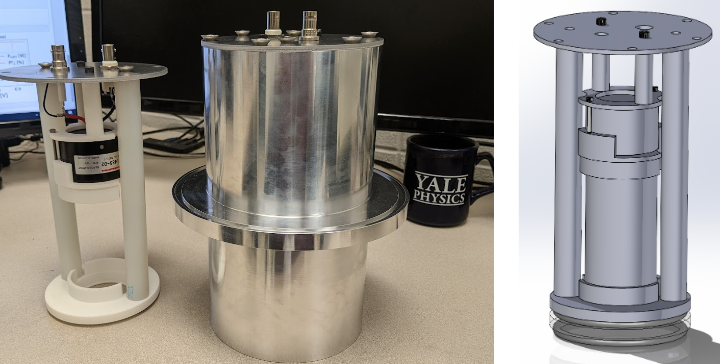
\includegraphics[width=\textwidth]{figs/todo/reentrant.png}
    \caption{Reentrant flange for lens testing detection chamber.}
    \label{reentrant}
\end{figure}

\begin{figure}
    \centering
    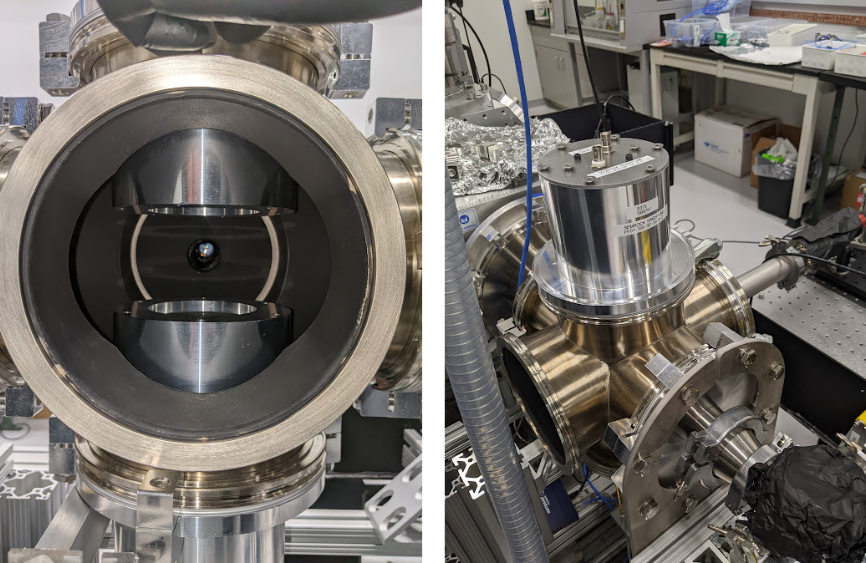
\includegraphics[width=\textwidth]{figs/todo/det_cross.png}
    \caption{Reentrant flanges in a `cross' vacuum chamber.}
    \label{det_cross}
\end{figure}

\begin{figure}
    \centering
    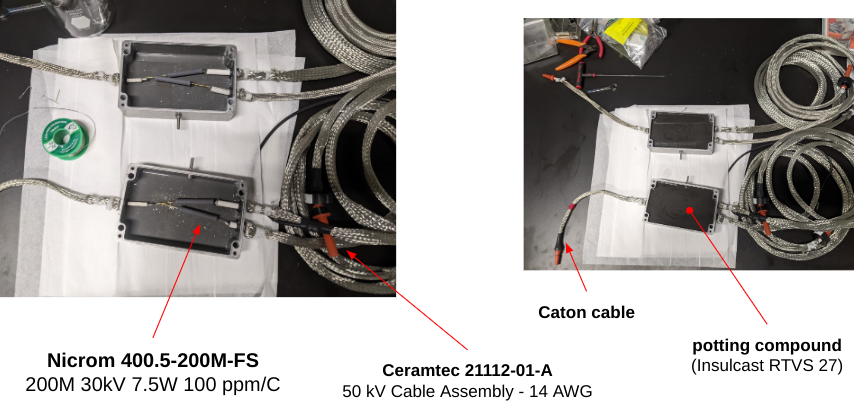
\includegraphics[width=\textwidth]{figs/todo/splitters.png}
    \caption{`Splitter' boxes for lens high voltage connections.}
    \label{splitters}
\end{figure}

\subsubsection{X-ray monitoring}
